\documentclass{article}

\usepackage{tikz}
\usepackage{rotate}

\usetikzlibrary{%
  arrows,%
  shapes.misc,% wg. rounded rectangle
  shapes.arrows,%
  chains,%
  matrix,%
  positioning,% wg. " of "
  scopes,%
  decorations.pathmorphing,% /pgf/decoration/random steps | erste Graphik
  shadows%
}

\begin{document}

\tikzset{
  nonterminal/.style={
    % The shape:
    rectangle,
    % The size:
    minimum size=12mm,
    % The border:
    very thick,
    draw=red!50!black!50,         % 50% red and 50% black,
                                  % and that mixed with 50% white
    % The filling:
    top color=white,              % a shading that is white at the top...
    bottom color=red!50!black!20, % and something else at the bottom
    % Font
    font=\itshape
  },
  terminal/.style={
    % The shape:
    rounded rectangle,
    minimum size=6mm,
    % The rest
    very thick,draw=black!50,
    top color=white,bottom color=black!20,
    font=\ttfamily},
  skip loop/.style={to path={-- ++(0,#1) -| (\tikztotarget)}}
}

{
  \tikzset{terminal/.append style={text height=1.5ex,text depth=.25ex}}
  \tikzset{nonterminal/.append style={text height=1.5ex,text depth=.25ex}}
}


\begin{tikzpicture}[
        point/.style={coordinate},>=stealth',thick,draw=black!50,
        tip/.style={->,shorten >=0.007pt},every join/.style={rounded corners},
        hv path/.style={to path={-| (\tikztotarget)}},
        vh path/.style={to path={|- (\tikztotarget)}},
        text height=1.5ex,text depth=.25ex % align text horizontally
    ]
    \matrix[column sep=4mm] {
        % First row:
        & & & & & & &  & & & & \node (plus) [terminal] {+};\\
        % Second row:
        \node (p1) [point] {}; & \node (ui1) [nonterminal] {unsigned integer};&
        \node (p2) [point] {}; & \node (dot) [terminal]    {.};               &
        \node (p3) [point] {}; & \node (digit) [terminal]    {digit};         &
        \node (p4) [point] {}; & \node (p5)  [point]  {};                     &
        \node (p6) [point] {}; & \node (e)   [terminal]    {E};               &
        \node (p7) [point] {}; &                                              &
        \node (p8) [point] {}; & \node (ui2) [nonterminal] {unsigned integer};&
        \node (p9) [point] {}; & \node (p10) [point]       {};\\
        % Third row:
        & & & & & & &  & & & & \node (minus)[terminal] {-};\\
    };

    { [start chain]
        \chainin (p1);
        \chainin (ui1)   [join=by tip];
        \chainin (p2)    [join];
         \chainin (dot)   [join=by tip];
        \chainin (p3)    [join];
        \chainin (digit) [join=by tip];
        \chainin (p4)    [join];
        { [start branch=digit loop]
        \chainin (p3) [join=by {skip loop=-6mm,tip}];
        }
        \chainin (p5)    [join,join=with p2 by {skip loop=6mm,tip}];
        \chainin (p6)    [join];
        \chainin (e)     [join=by tip];
        \chainin (p7)    [join];
        { [start branch=plus]
        \chainin (plus)  [join=by {vh path,tip}];
        \chainin (p8)    [join=by {hv path,tip}];
        }
        { [start branch=minus]
        \chainin (minus) [join=by {vh path,tip}];
        \chainin (p8)    [join=by {hv path,tip}];
        }
        \chainin (p8)    [join];
        \chainin (ui2)   [join=by tip];
        \chainin (p9)    [join,join=with p6 by {skip loop=-11mm,tip}];
        \chainin (p10)   [join=by tip];
  }
\end{tikzpicture}

\begin{tikzpicture}[
        point/.style={coordinate},>=stealth',thick,draw=black!50,
        tip/.style={->,shorten >=0.007pt},every join/.style={rounded corners},
        text height=1.5ex,text depth=.25ex % align text horizontally
]

\matrix[row sep=3mm,column sep=2mm] {
% First row
& & \node (atom1) [nonterminal,yshift=12mm] {\begin{tabular}{l} Use New and Existing \\ Allele Associations \end{tabular}}; & & \\
& \node (yes1) [terminal] {Yes}; & & & \\
% Second row
\node (atom2) [nonterminal] {\begin{tabular}{l} New Allele \\ Associations? \end{tabular}}; & & & & \node (atom3) [nonterminal] {\begin{tabular}{l} Use Epitope Prediction \\ To Discover Properties \\ of Beneficial Alleles \end{tabular}}; \\
& \node (no1) [terminal] {No}; & & & \\
% Third row
& & \node (atom4) [nonterminal,yshift=-12mm] {\begin{tabular}{l} Use Existing \\ Allele Associations \end{tabular}}; & & \\
\\

\node (atom5) [nonterminal] {\begin{tabular}{l}  Test and Modify \\ Existing Epitope \\ Prediction Software \end{tabular}}; & & \node (atom6) [nonterminal] {\begin{tabular}{l}  Test Adapted \\ Epitope Prediction \\ Software \end{tabular}}; & & \node (pos1) [point] {.};\\
\node (atom7) [nonterminal] {\begin{tabular}{l} Modelling CTL lysis \\ with Tax Expression \end{tabular}}; & & \node (atom8) [nonterminal] {\begin{tabular}{l}  How Does Antigen \\ Expression Affect \\ CTL Killing? \end{tabular}}; & & \\
};

{ [start chain]

	\chainin (atom2);
        \chainin (yes1)   [join=by tip];


}


\end{tikzpicture}




\begin{center}
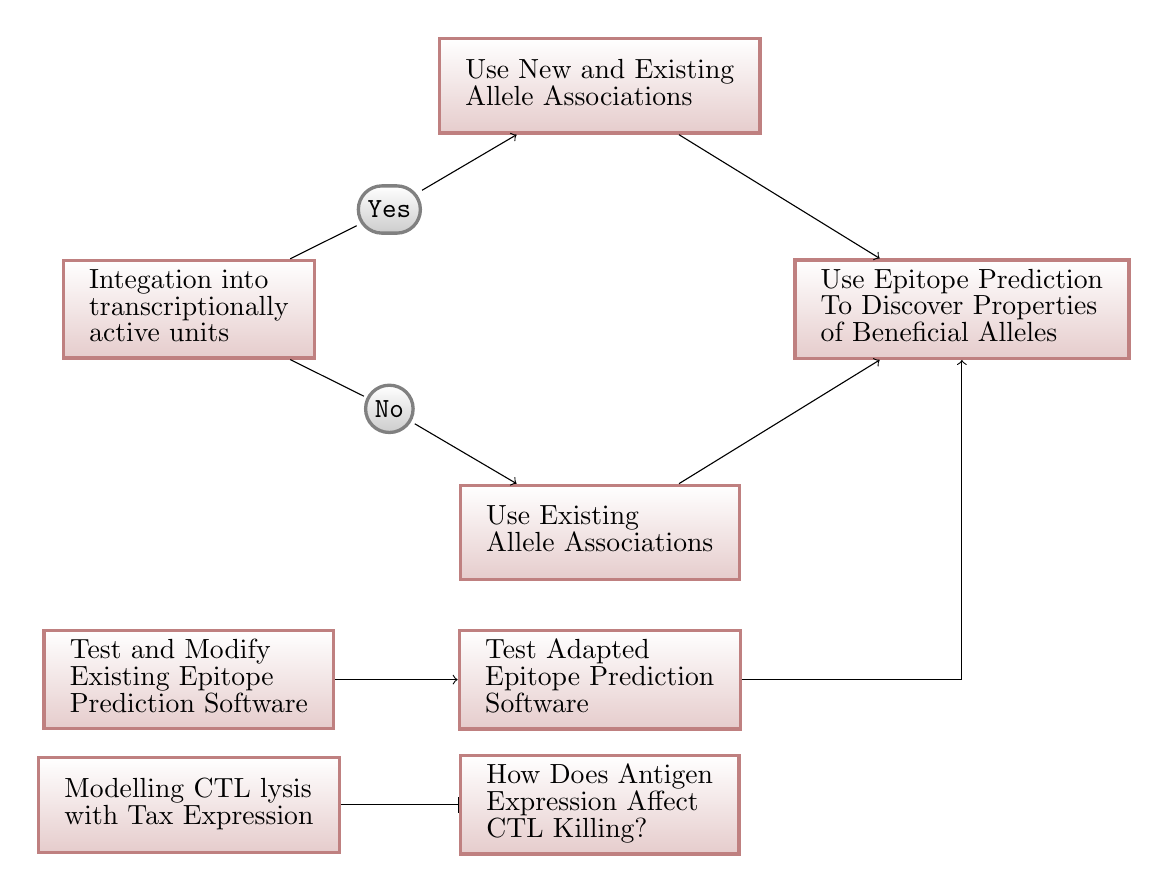
\begin{tikzpicture}[nonterminal/.style={
	rectangle,
	minimum size=12mm,
	very thick,
	draw=red!50!black!50, 
	top color=white, 
	bottom color=red!50!black!20
%	font=\itshape
	},terminal/.style={
	rectangle,minimum size=6mm,rounded corners=3mm,
	very thick,draw=black!50,
	top color=white,bottom color=black!20,
	font=\ttfamily
	},point/.style={
	coordinate,thick,draw=black!50
	}
%	Need to check these with chain	
%	 ,tip/.style={
%	->,shorten >=1pt
%	},every join/.style={
%	rounded corners
%	},hv path/.style={
%	to path={-| (\tikztotarget)}
%	},vh path/.style={
%	to path={|- (\tikztotarget)}
%	}
]

\matrix[row sep=3mm,column sep=2mm] {
% First row
& & \node (atom1) [nonterminal,yshift=9.5mm] {{\renewcommand{\arraystretch}{0.75}\begin{tabular}{l} Use New and Existing \\ Allele Associations \end{tabular}}}; & & \\
& \node (yes1) [terminal] {Yes}; & & & \\
% Second row
\node (atom2) [nonterminal] {{\renewcommand{\arraystretch}{0.75}\begin{tabular}{l} Integation into \\ transcriptionally \\ active units \end{tabular}}}; & & & & \node (atom3) [nonterminal] {{\renewcommand{\arraystretch}{0.75}\begin{tabular}{l} Use Epitope Prediction \\ To Discover Properties \\ of Beneficial Alleles \end{tabular}}}; \\
& \node (no1) [terminal] {No}; & & & \\
% Third row
& & \node (atom4) [nonterminal,yshift=-9.5mm] {{\renewcommand{\arraystretch}{0.75}\begin{tabular}{l} Use Existing \\ Allele Associations \end{tabular}}}; & & \\
\\

\node (atom5) [nonterminal] {{\renewcommand{\arraystretch}{0.75}\begin{tabular}{l} Test and Modify \\ Existing Epitope \\ Prediction Software \end{tabular}}}; & & \node (atom6) [nonterminal] {{\renewcommand{\arraystretch}{0.75}\begin{tabular}{l} Test Adapted \\ Epitope Prediction \\ Software \end{tabular}}}; & & \node (pos1) [point] {.};\\
\node (atom7) [nonterminal] {{\renewcommand{\arraystretch}{0.75}\begin{tabular}{l} Modelling CTL lysis \\ with Tax Expression \end{tabular}}}; & & \node (atom8) [nonterminal] {{\renewcommand{\arraystretch}{0.75}\begin{tabular}{l} How Does Antigen \\ Expression Affect \\ CTL Killing? \end{tabular}}}; & & \\
};

%	chain not working, try again if you have time

\path	(atom2)	edge[-] (yes1)
	(atom2) edge[-] (no1)
	(yes1) 	edge[->] (atom1)
	(no1) 	edge[->] (atom4)
	(atom1) edge[->] (atom3)
	(atom4) edge[->] (atom3);
\path	(atom5) edge[->] (atom6)
	(atom6) edge[-] (pos1)
	(pos1) 	edge[->] (atom3);
\path	(atom7) edge[-|] (atom8);

\end{tikzpicture}[line width=20pt]
\end{center}

\begin{center}
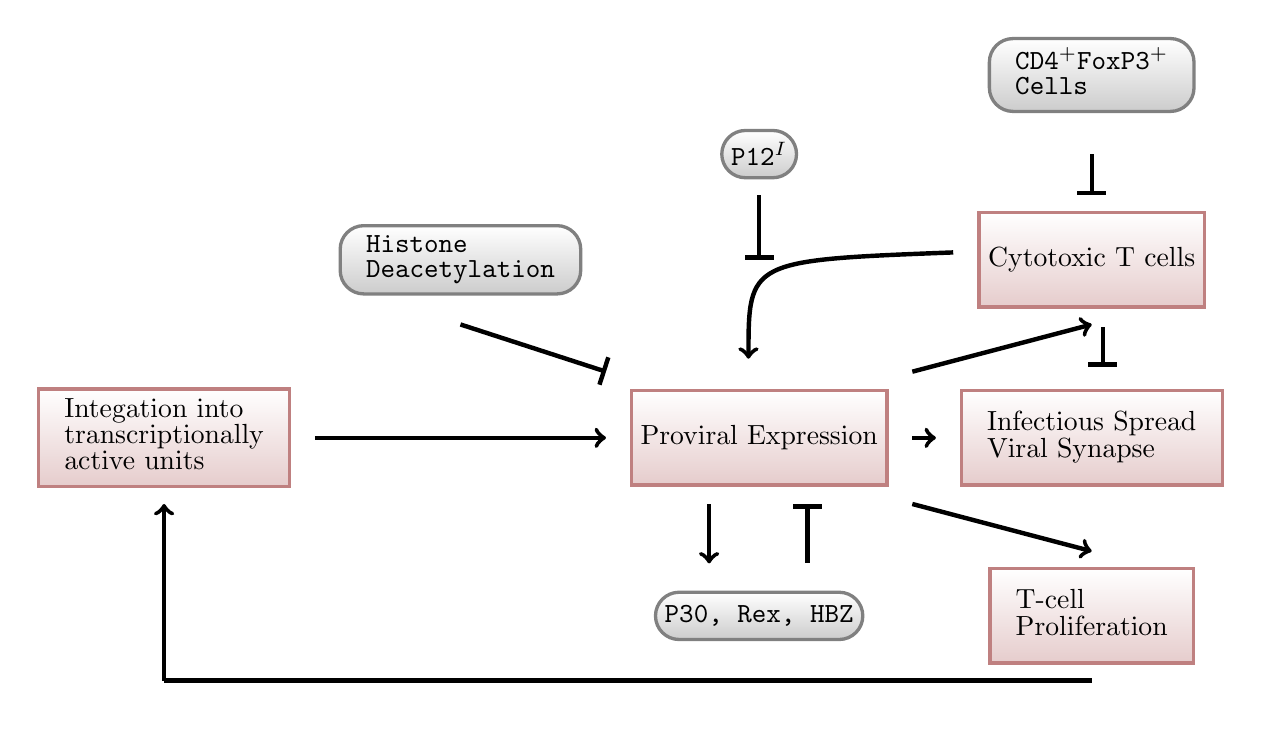
\begin{tikzpicture}[nonterminal/.style={
	rectangle,
	minimum size=12mm,
	very thick,
	draw=red!50!black!50, 
	top color=white, 
	bottom color=red!50!black!20
%	font=\itshape
	},terminal/.style={
	rectangle,minimum size=6mm,rounded corners=3mm,
	very thick,draw=black!50,
	top color=white,bottom color=black!20,
	font=\ttfamily
	},point/.style={
	circle,inner sep=0pt,minimum size=2pt,fill=red
	},point1/.style={
	coordinate,thick,draw=black!50
	}
]

\matrix[row sep=2mm,column sep=3mm] {
& & & & & & & \node (atom3) [terminal] {{\renewcommand{\arraystretch}{0.75}\begin{tabular}{l} CD4$^+$FoxP3$^+$ \\ Cells \end{tabular}}};
\\
 &  &  &  & \node (atomP12) [terminal] {P12$^I$}; &  &  & \node (POSP) [point1] {.}; \\
 &  &  &  & \node (POSY) [point1] {.}; &  &  & \node (POSQ) [point1] {.}; \\
% First row
 &  & \node (atomHIS) [terminal] {{\renewcommand{\arraystretch}{0.75}\begin{tabular}{l} Histone \\ Deacetylation \end{tabular}}}; &  & \node (POSZ) [point1] {.}; &  & \node (POSO) [point1] {.}; & \node (atomCTL) [nonterminal] {Cytotoxic T cells}; \\
 &  & \node (POSI) [point1] {.}; &  &  &  &  & \node (POSF) [point1] {.}; \\
 &  &  &  &  &  &  &  \\
 &  &  &  &  &  &  &  \\
 &  &  & \node (POSJ) [point1] {.}; & \node (POSN) [point1] {.}; & \node (POSE) [point1] {.}; &  &  \\
% Second row
\node (atom1) [nonterminal] {{\renewcommand{\arraystretch}{0.75}\begin{tabular}{l} Integation into \\ transcriptionally \\ active units \end{tabular}}}; & \node (POSA) [point1] {.}; &  & \node (POSB) [point1] {.}; & \node (atom2) [nonterminal] {Proviral Expression}; & \node (POSC) [point1] {.}; & \node (POSD) [point1] {.}; & \node (atom3) [nonterminal] {{\renewcommand{\arraystretch}{0.75}\begin{tabular}{l} Infectious Spread \\ Viral Synapse \end{tabular}}};\\
\node (POSM) [point1] {.}; &  &  &  & \node (POSR) [point1] {.}; & \node (POSG) [point1] {.}; &  &  \\
 &  &  &  &  &  &  &  \\
 &  &  &  &  &  &  &  \\
 &  &  &  & \node (POSS) [point1] {.}; &  &  & \node (POSH) [point1] {.}; \\
% Third row
 &  &  &  & \node (atomProt) [terminal] {P30, Rex, HBZ}; &  &  & \node (atomProl) [nonterminal] {{\renewcommand{\arraystretch}{0.75}\begin{tabular}{l} T-cell \\ Proliferation \end{tabular}}};\\
\node (POSK) [point1] {.}; &  &  &  &  &  &  & \node (POSL) [point1] {.}; \\
\\
};

%	chain not working, try again if you have time

%(x,y)
\draw[->, ultra thick] (4.1,1.45) .. controls (1.5,1.35) .. (1.5,0.1);
\draw[ultra thick]	(POSA) edge[->] (POSB);
\draw[ultra thick]	(POSC) edge[->] (POSD);
\draw[ultra thick]	(POSE) edge[->] (POSF);
\draw[ultra thick]	(POSG) edge[->] (POSH);
\draw[ultra thick]	(POSI) edge[-|] (POSJ);
\draw[ultra thick]	(POSK) edge[-] (POSL);
\draw[ultra thick]	(POSK) edge[->] (POSM);
%\draw[ultra thick]	(POSN) edge[|-] (POSO);
\draw[ultra thick]	(POSP) edge[-|] (POSQ);
\draw[ultra thick]	(POSY) edge[-|] (POSZ);
\draw[->, ultra thick] (1,-1.75) -- (1,-2.5);
\draw[|-, ultra thick] (2.25,-1.75) -- (2.25,-2.5);
\draw[-|, ultra thick] (6,0.5) -- (6,0);








%\draw[ultra thick]	(atom2) edge[->] (atom3);
%\draw[ultra thick]	(atom2) edge[->] (atomCTL);
%\draw[ultra thick]	(atom2) edge[->] (atomProl);
%\draw[ultra thick]	(atom2) edge[|->] (atomProt);
%\draw[ultra thick]	(atomCTL) edge[-] (posA);
%\draw[ultra thick]	(posA) edge[-|] (atom2);
%\draw[ultra thick]	(atomP12) edge[-|] (posA);
%\draw[ultra thick]	(atomHIS) edge[-|] (atom2);





\end{tikzpicture}
\end{center}

\end{document}















































